\chapter{APRS Background and Definitions}
From the introduction it is known that APRS is a method of digital communication used by hams in order to inform other hams of their location. In addition to supporting sending positions, APRS can be used to send messages, bulletins, weather, and other information. Since these packets are transmitted via radio  - which has limited coverage - APRS can be viewed as a local area awareness network. This gives hams who are listening for and decoding APRS packets information about nearby transmitting stations. This brief overview should give a little insight into APRS, but the rest of the section will focus more on what is going on behind-the-scenes to explain how APRS works in terms of the protocols, data transmission, modulation, etc.

In order to organize this discussion of the different components of APRS let us break it down into the Open Systems Interconnection (OSI) model representation. However, before fitting it into the OSI model here is a brief reminder of the relevant layers that are going to be discussed. Layer 1 of the OSI model is the physical layer. The physical layer consists of everything that is used to transport one bit of information from one location to another. The second layer is the data link layer. Within the data link layer bits from the physical layer are passed up to the network layer, and information from the network layers is framed and handed off to the physical layer. Layer 3 is the Networking layers. This Layer is responsible for determining the path that packets will take and providing flow control to prevent flooding. Above these layers are layers 4-7 which are the transport, session, presentation, and application layers respectively \cite{Sosinsky2009}. These upper layers get too inter-tangled to be able to cleanly separate them. For instance within the AX.25 2.2 specification a TNC is mentioned that only implements layers 1, 2, and 7 of the OSI model \cite{Beech1998}.

Here is the best division of APRS into the OSI model, following introducing this division each layer will be individually discussed in more detail. Layer 3 of the OSI model for APRS is the the AX.25 Protocol,  High-Level Data Link Control (HDLC) protocol composes layer 2. All the way at the bottom, layer 1 for APRS consists of the Terminal Node Controller (TNC) and Radio \cite{Silver2013}. A brief note on why the discussion begins with Layer 3 is because this is how the data is transferred. The interest stop here and does not continue to the layers above layer three, because those are all application specific. Starting with AX.25 the background information will be given down to Layer 1 which is where this research actually aims to make a contribution.

\section{Layer 3 - AX.25}
Layer 3, the network layer, is responsible for routing frames between individual nodes in the network. A frame of data is more traditionally called a packet at this point since AX.25 is a packet switched network protocol \cite{Peterson2011}. AX.25 is the amateur X.25 protocol. Meaning that the AX.25 protocol, which is what APRS uses, was developed my Amateur radio operators and is based off of the x.25 protocol. Since the origins of AX.25 lie within X.25, the discussion will begin with X.25. 

\subsection{X.25}
Developed in the 1970s the packet switching protocol X.25 was deployed on telephone networks where it was used until it began to be displaced by the IP protocol. The X.25 protocol suite provides OSI layers 1-3, although it does have standards that support each of those layers \cite{Sosinsky2009}. For instance the X.21 standard is commonly used for layer 1 of X.25 and ISO 7776 specifies a Link Access Procedure Balanced (LAPB) to assists with layer 2, the data link layer \cite{Gallagher1997}. The Data Link layer of LAPB, a bit oriented protocol derived of HDLC,  manages packet framing and ensures that frames are error free and properly sequenced. When used on telephone networks there were five distinct modes that the protocol would operate in: Call setup for establishing the connection, Data transfer, idle where the connection is established but no data is being transferred, call clearing for terminating the connection, and restart for resynchronizing the host and client \cite{Javvin2006}. Many of the features of the Layer 2 and Layer 3 operations of X.25 can be found in at least a similar fashion in AX.25.

\subsection{AX.25}
Next the AX.25 protocol will be discussed through comparison and contrast with X.25. One of the main differences between the X.25 and AX.25 is that when the specification is read, in addition to specifying the behavior of Layer 3, the behavior of Layer 2 is also included. Although this is somewhat implied for X.25, there are still separate documents for the specifications for each one of the layers. After reading the specification for AX.25 it very clearly defines the framing with starting and terminating flags as well as the networking and routing \cite{Beech1998}.

\section{Layer 2 - High-Level Data Link Control}
Layer 2 of the OSI model which is responsible for framing the bits, or packets, from layer 3 is taken on my HDLC in APRS. The goal of HDLC is to make sure that when the data is received and passed up to Layer 3, that it is error free, without loss, and in the correct order \cite{Javvin2006}. There are a few ways that HDLC accomplishes this, two of which are framing and with the Frame Check Sequence (FCS). The framing occurs through the use of flags around the data. A flag is one byte and is hex 0x7E. For APRS common practice is to send multiple flags consecutively to give transmitting radio time to key up and settle or to give receiving radios time for their squelch to open. Since it is an non-return to zero inverted (NRZI) encoding no change in frequency corresponds to a 1 and a change in frequency corresponds to a 0. As such multiple 1s in a row make it hard to keep timing which is why bit stuffing is used. With the exception of the flag which contains six consecutive 1s (0x7E = 01111110) if there six or more consecutive 1s in the data packet a zero will be stuffed after the fifth 1 to increase the clocking energy in the signal.

\section{Layer 1 - The Bell 202 Modulation and the Radio}
Since Layer one is composed of the things needed in order to transmit one bit from one location to another, it needs to be made clear what all this includes for APRS. Starting with air, the medium through which the radio frequency (RF) signals propagate, the RF transmissions are received or transmitted by the radio. Without decomposing the radio into all of its individual components, the audio that the radio receives then has to be processed. In order to stay focused on what happens in layer 1 and not start mixing the other layers together some more discussion of what this audio signal consists of is necessary.

The audio signal that contains the APRS packets is composed using the Bell 202 modulation which is an Audio Frequency Shift Keying (AFSK) mode. As such RF either comes in through the radio, is translated to the corresponding audio, and then demodulated into a bit stream by interpreting the Bell 202 modulation. Or, a bit stream from layer 2 of APRS is modulated using the Bell 202 modulation, this modulated audio is passed to the radio, and the radio then transmits it out. Since decomposing the radio down into its individual components does not have any affect on representing the different OSI layers of APRS, it will not be discussed. However there are factors that affect wireless communications and RF signals that will be discussed in chapter 4.

\subsection{Frequency Shift Keying}
In order to understand the Bell 202 modulation scheme the communication mode of AFSK needs to be introduced. AFSK is a form of frequency shift keying (FSK) that occurs by modulating frequencies in the audible range. FSK uses multiple frequencies in order to represent the different symbols such as 1 or 0 or mark and space in our case. If the frequency of the data carrying signal can be determined, then the symbol is knows for that bit period. FSK is the more generic term and is used for 9600 baud (bits per second) APRS on Ultra High Frequencies (UHF). In this mode the actual RF carrier in the 440MHz band is modulated between one frequency and another nearby frequency in order to represent the two different symbols. In contrast, AFSK switches between two different audio signals, which for APRS on Very High Frequencies (VHF) is then modulated onto the RF carrier using Frequency Modulation (FM).


\subsection{Bell 202}
With FSK and AFSK now introduced the AFSK used within Bell 202 can be described. The Bell 202 modem was patented in 1984 using 1200Hz and 2200Hz tones, although the patent was originally filed in 1981 \cite{stauffer1984fsk}. Interestingly, the International Telecommunication Union (ITU) did not publish a standard for this modulation that were used in telephone networks until 1988. In the standard, however they use 1300Hz tone for symbol 1 and 2100Hz tone for symbol 2 called a mark and space respectively \cite{ITUV23}. The original bit stream is modulated using a non-return to zero inverted (NRZI) encoding. This means that when a transition occurs from one symbol to another in the Bell 202 modulated signal this symbolizes a 0 bit in the original data bit stream and if the Bell 202 symbol remains constant over multiple symbol periods, that signifies a 1 bit in the original data bit stream. For Bell 202 the frequencies that are used are 1200Hz and 2200Hz tones for the mark and the space as opposed to the 1300Hz and 2100Hz tones proposed in the ITU specification.
\begin{Figure}
  \centering
	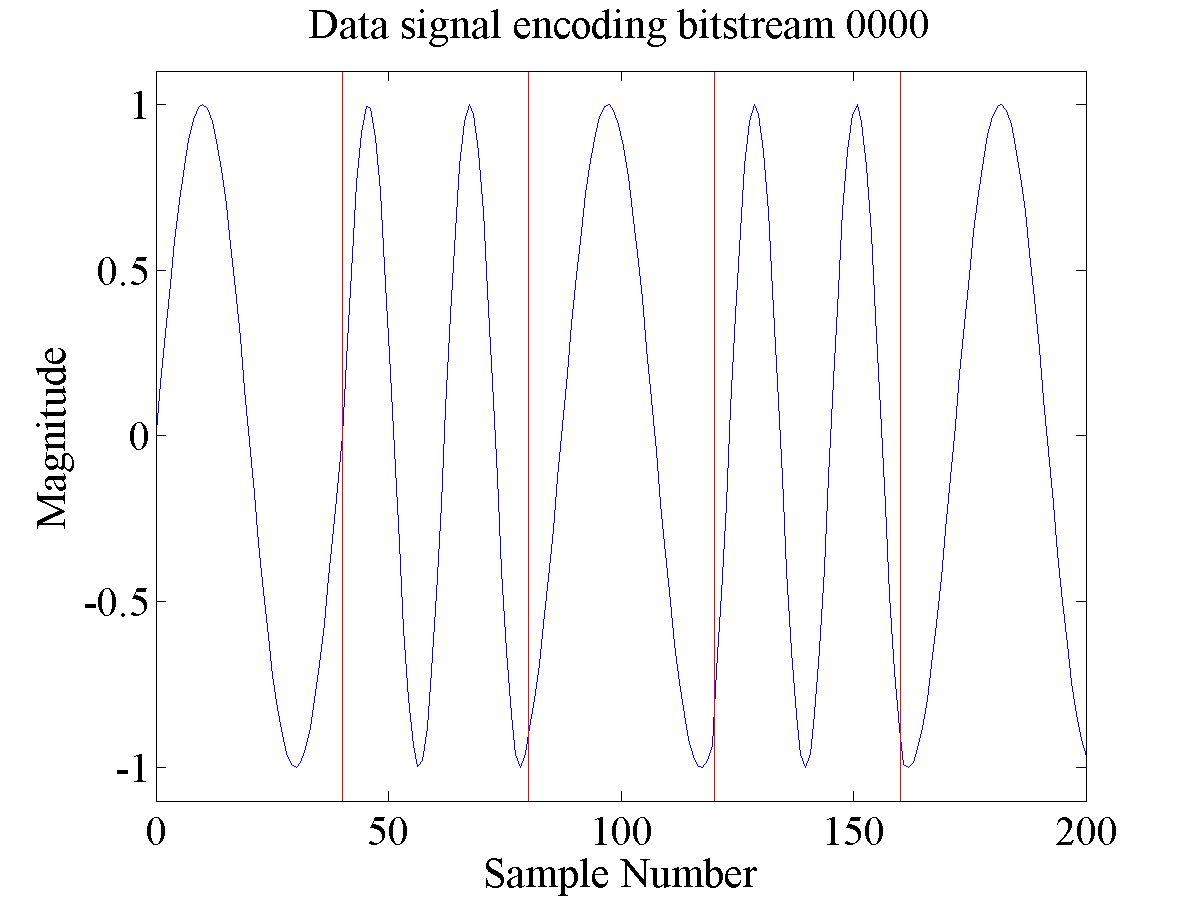
\includegraphics[width=0.75\linewidth]{Datasignalencodingbitstream0000.png} 
	\captionof{figure}{Example Bell 202 signal encoding the bit stream '0000'.}
\end{Figure}